\documentclass[12pt,a4paper]{report}
\usepackage[french]{babel}
\usepackage[utf8]{inputenc}
\usepackage[T1]{fontenc}
\usepackage[justification=centering]{caption}
\usepackage{lmodern}
\usepackage{graphicx} 
\usepackage{geometry}
\usepackage{hyperref}
\usepackage{csquotes}
\usepackage{multirow}
\usepackage{fancyvrb}
\usepackage{svg}
\usepackage{amsmath}
\usepackage{placeins}
\usepackage{float}
\usepackage{stmaryrd}
\usepackage{framed}
\usepackage{tcolorbox}
\usepackage{subcaption} 
\usepackage{algpseudocode}
\usepackage{algorithm}
\usepackage{array} 
\usepackage{tabularx}
\usepackage{booktabs}
\usepackage[export]{adjustbox} 
\usepackage{lipsum}
\usepackage{caption} 
\usepackage{listings}
\usepackage{xcolor}
\usepackage{pdflscape}
\usepackage{makecell}

% Configuration de la mise en page
\geometry{left=2.5cm, right=2.5cm, top=2.5cm, bottom=2.5cm}

\usepackage[style=authoryear, backend=biber, maxbibnames=99]{biblatex}
\addbibresource{references.bib}
\usepackage{hyperref}

% Custom citation formatting
\renewcommand*{\nameyeardelim}{\addcomma\space}
\DeclareFieldFormat{cite}{\mkbibparens{\citeyear{#1}}}



\begin{document}

\begin{titlepage}

\centering
\begin{figure}[ht]
    \centering           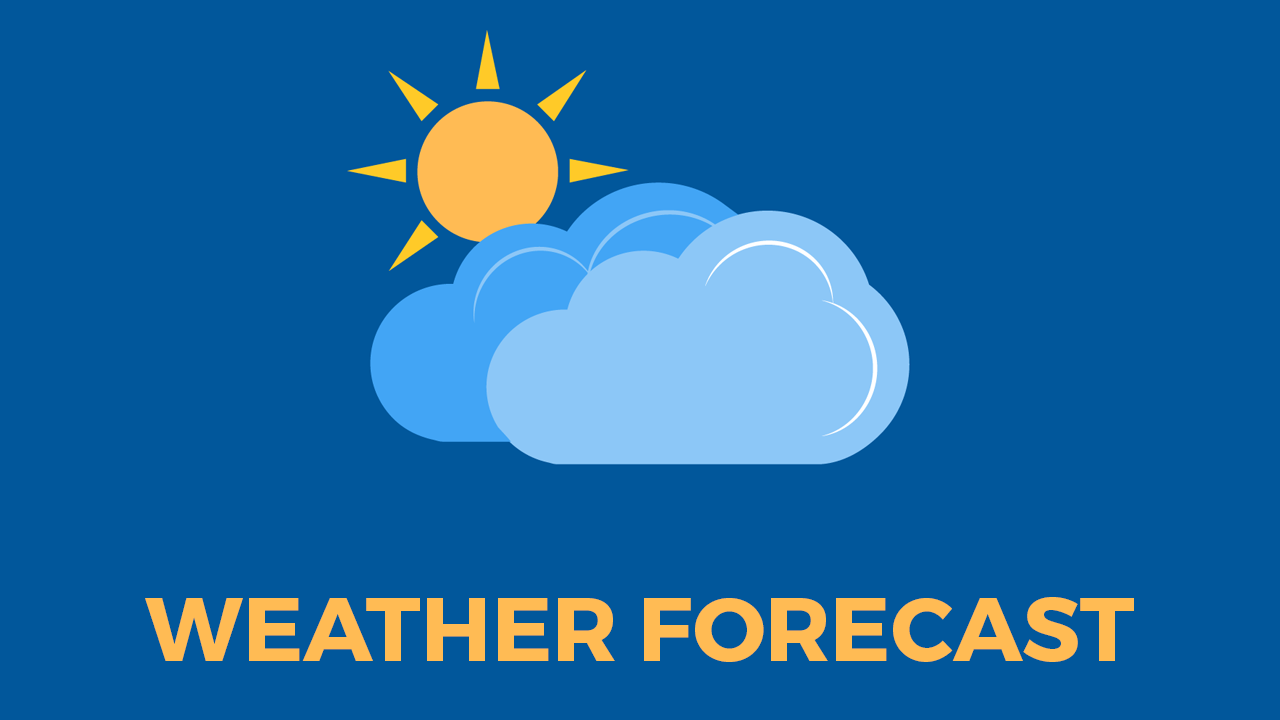
\includegraphics[width=0.9\textwidth]{media/weather-forecast.png}
\end{figure}

\vspace{-0.5cm}

\begin{center}
    \rule{\linewidth}{0.5pt} % Horizontal line
    \vspace{0.5cm}
    {\Large\bfseries Internship Report \par}
    {\Large\bfseries Local Machine Learning-based weather prediction \par}
    \rule{\linewidth}{0.5pt} % Horizontal line
\end{center}

\vspace{0.5cm}

{\large Gwendal SALIOU \par}
{\large\today\par}

\vfill
\begin{tabular}{cccc}
    
\includegraphics[width=3cm]{media/logo_IMT.png} \hspace{1cm} &
    
\includegraphics[width=8cm]{media/logo_riken.png} \hspace{1cm} &
    
\includegraphics[width=3cm]{media/logo_IUEM.png} \\
\end{tabular}
\null

\end{titlepage}
\newpage



% Tables des matières
\tableofcontents
\newpage


\chapter{Introduction}

For the past decade, numerical weather prediction (NWP) has been the primary approach for weather forecasting. NWP involves the numerical integration of partial differential equations, starting from the best estimate of the current state of the Earth system, to produce a weather forecast. In a standard NWP framework, a weather prediction is obtained through a deductive inference process, where the laws of physics are used to derive a deterministic forecast from the best possible initial conditions. These initial conditions are obtained by optimally combining Earth system observations and short-range forecasts through a process known as \textit{data assimilation}.\\

However, the Earth's state can never be known perfectly, and to account for this, \textit{ensemble forecasting} is often used. This involves making multiple forecasts with small perturbations from a Gaussian distribution around the uncertainties in the system. While NWP has seen significant improvements in recent years, the biggest drawback is still the computational resources required to make accurate predictions in an operational context.\\

Limited area modeling is crucial as it allows for high-resolution forecasts over specific regions without the need to model the entire globe, thereby significantly reducing computational costs. By focusing computational resources on a smaller area, limited area models (LAMs) can provide more detailed and accurate forecasts for local regions, which is essential for applications such as severe weather warnings, local climate studies, and resource management. Additionally, to compute high-resolution forecasts, high-resolution data are required. Currently, the best resolution available for a global forecast is 0.25°.\\

In this context, data-driven modeling based on machine learning (ML) is showing great potential for weather forecasting applications. ML-based models offer the promise of delivering forecasts at a much lower computational cost, along with potential benefits such as increased timeliness and potentially increased accuracy.\\

The aim of this project is to develop a local weather forecasting framework based on machine learning (ML) techniques using historical data from the ERA5 dataset. To achieve this goal, an initial approach will be devised that involves inputting two types of data into our system:\\

\begin{itemize}
    \item The low-resolution state of our system at time \( t + \Delta t \), which can initially be obtained from the ERA5 dataset. In the context of actual forecasting, these data can subsequently be replaced by a global model.
    \item The high-resolution spatial state of our system at times \( t \) and \( t - \Delta t \) over a local range (e.g., 0.25° of latitude by 0.25° of longitude).
\end{itemize}

\vspace{2em}

By utilizing these two types of data, we aim to predict local weather conditions at time \( t + \Delta t \) with higher resolution than the global state and create a proof of concept for a higher resolution forecast for a limited area. To accomplish this, ML techniques will be employed to train our forecasting model using historical data. The performance of our model will then be evaluated using WeatherBench2 \cite{Weatherbench}.


\section{Dataset}

\section{Dataset}

ERA5 is a meteorological and climatological dataset provided by the European Centre for Medium-Range Weather Forecasts (ECMWF). It is a reanalysis dataset that combines model data with observations from around the world to create a globally complete and consistent dataset. ERA5 provides hourly estimates for a wide range of atmospheric, ocean-wave, and land-surface quantities, along with an uncertainty estimate. The dataset is available from 1940 onwards and is updated daily with a delay of approximately five days. 

The data is regridded onto a regular lat-lon grid of 0.25 degrees for reanalysis and 0.5 degrees for uncertainty estimation. The time step between two system states is 1 hour. ERA5 is the primary dataset used by Machine Learning-based Weather Prediction (MLWP) systems.



\section{How do we use the data}

\subsection{Train test validation}

For the period I suggest that we take as KARINA and other model did which is the years 1979 to 2015 for training, 2016 and 2017 are for validation and 2018 as formal test. The choice to take data from 1979 onwards is three fold : first it correspond to the state of the art models choices, secondly it is the most recent years and it has been shown (show citation) that the models output might need the most recent years to make the best forecast and account for global warming trend and third the data before 1979 is said to be less trustworthy at this resolution.\\

\subsection*{For the local model}

We want the regional model to cover an area of 3000 km by 2000 km, which represents approximately 30 degrees by 20 degrees. With a resolution of 0.25 degrees for our data, this corresponds to a grid of approximately 120 by 80. We might choose 37 pressure level as graphCast did for the high resolution state. We will take from 30 to 50 N° and 125 to 155 E°.\\

We will take 66 variables consisting of six surface variables and five variables with 12 vertical pressure levels from the surface to the lower stratosphere, known as prognostic variables of the Earth’s atmosphere. Accordingly with the study of  \cite{cheon2024advancing} we will use the following variables and the orography:\\

\begin{table}[!h]
	\caption{Comprehensive List of Key Atmospheric Variables for Climate Modeling, Corresponding Short Names, Vertical Measurement Levels hPa), and Units.}
	\centering
    \scriptsize
	\begin{tabularx}{\textwidth}{@{}lXXXX@{}}
		\toprule
		Variable name & Short name & Vertical levels (hPa) & Units & \\
		\midrule
		Zonal wind & U & 1000, 925, 850, 800, 700, 600, 500, 400, 300, 200, 100, 50 & m/s & \\
		\addlinespace
		Meridional wind & V & 1000, 925, 850, 800, 700, 600, 500, 400, 300, 200, 100, 50 & m/s & \\
		\addlinespace
		Temperature & T & 1000, 925, 850, 800, 700, 600, 500, 400, 300, 200, 100, 50 & K & \\
		\addlinespace
		Specific humidity & Q & 1000, 925, 850, 800, 700, 600, 500, 400, 300, 200, 100, 50 & kg/kg & \\
		\addlinespace
		Geopotential & Z & 1000, 925, 850, 800, 700, 600, 500, 400, 300, 200, 100, 50 & m\(^2\)/s\(^2\) & \\
		\addlinespace
		2m temperature & T2m & & K & \\
		\addlinespace
		Mean sea level pressure & MSL & & Pa & \\
		\addlinespace
		Surface air pressure & SP & & Pa & \\
		\addlinespace
		Total column vertically-integrated water vapour & TCWV & & kg/m\(^2\) & \\
		\addlinespace
		Skin temperature & SKT & & K & \\
		\addlinespace
		TOA incident solar radiation & TISR & & J/m\(^2\) & \\
		\bottomrule
	\end{tabularx}
	\label{tab:variables}
\end{table}

It seems that we could do it that way but we have to check \href{https://cds.climate.copernicus.eu/cdsapp#!/dataset/reanalysis-era5-complete?tab=form}{here}: \\

For the query of all variables : 
\scriptsize
\begin{Verbatim}
    #!/usr/bin/env python
import cdsapi

c = cdsapi.Client()

c.retrieve("reanalysis-era5-complete", {
    "class": "ea",
    "date": "1979-12-01/to/2015-12-31",
    "expver": "1",
    "levtype": "sfc",
    "param": "134.128/137.128/151.128/165.128/167.128/235.128",  #165.128 TOA incident solar radiation
    "stream": "oper",
    "time": "00:00:00/01:00:00/02:00:00/03:00:00/04:00:00/05:00:00/06:00:00/07:00:00/
    08:00:00/09:00:00/10:00:00/11:00:00/12:00:00/13:00:00/14:00:00/15:00:00/16:00:00/
    17:00:00/18:00:00/19:00:00/20:00:00/21:00:00/22:00:00/23:00:00",
    "type": "an"
}, "output1")

c.retrieve("reanalysis-era5-complete", {
    "class": "ea",
    "date": "1979-12-01/to/2015-12-31",
    "expver": "1",
    "levelist": "50/100/200/300/400/500/600/700/800/850/925/1000",
    "levtype": "pl",
    "param": "129.128/130.128/131/132/133.128"
    "stream": "oper",
    "time": "00:00:00/01:00:00/02:00:00/03:00:00/04:00:00/05:00:00/06:00:00/07:00:00/
    08:00:00/09:00:00/10:00:00/11:00:00/12:00:00/13:00:00/14:00:00/15:00:00/16:00:00/
    17:00:00/18:00:00/19:00:00/20:00:00/21:00:00/22:00:00/23:00:00",
    "type": "an"
}, "output2")

\end{Verbatim}
\normalsize

\section{Model to Develop}

The aim of this internship is to develop a machine learning model that provides as output (\textbf{Y}) a regional-scale, high-resolution weather forecast, which will be referred to as High Resolution Local (\textbf{HRL}) in this document. Initially, the input (\textbf{X}) will be an HRL at time t, denoted as \textbf{HRL(t)}. This first model will represent a simple forecast. Subsequently, a low-resolution global model, referred to as Low Resolution Global (\textbf{LRG}), will be added to the input to potentially improve the system's predictions by providing context.

The work of \href{https://events.ecmwf.int/event/172/contributions/1769/attachments/877/1550/Machine-Learning-WS_Mdini.pdf}{Maha Mdini} should be analyzed to identify any ideas that could be incorporated into the future model.

\vspace{2em}

\begin{tabular}{>{\bfseries}l<{\hspace{1em}} >{\centering\arraybackslash}p{7cm} >{\raggedleft\arraybackslash}p{2cm}}
\hline
\textbf{Model to Develop} & \textbf{Input (X)} & \textbf{Output (Y)}\\
\hline
Model 1 & HRL(t) & HRL(t+dt) \\
Model 2 &  HRL(t) + LRG(t) & HRL(t+dt) \\
Model 3 &  HRL(t) + LRG(t) + LRG (t+dt) & HRL(t+dt) \\
Model 4 & autoregressive & HRL(t+dt) \\
\end{tabular}

\subsection{Model 1: Simple Forecast within a Region}

\begin{figure}[ht]
\centering
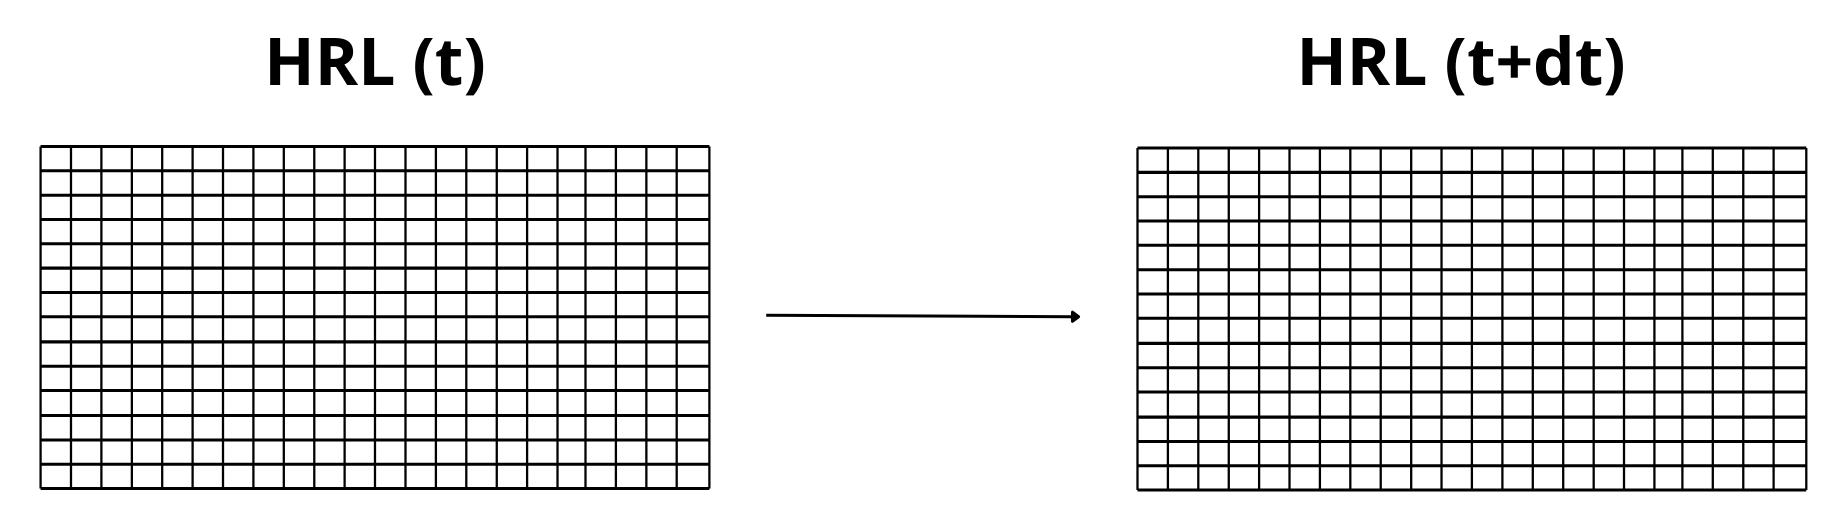
\includegraphics[width=0.9\textwidth]{media/model1.png}
\caption{Architecture of Model 1: Simple Forecast}
\label{fig}
\end{figure}

This model represents a simple forecast within a region with a known state at time t on a fine grid to obtain a known state at time t+dt on a fine grid.

\subsection{Model 2: Forecast with Boundary Conditions}

\begin{figure}[ht]
\centering
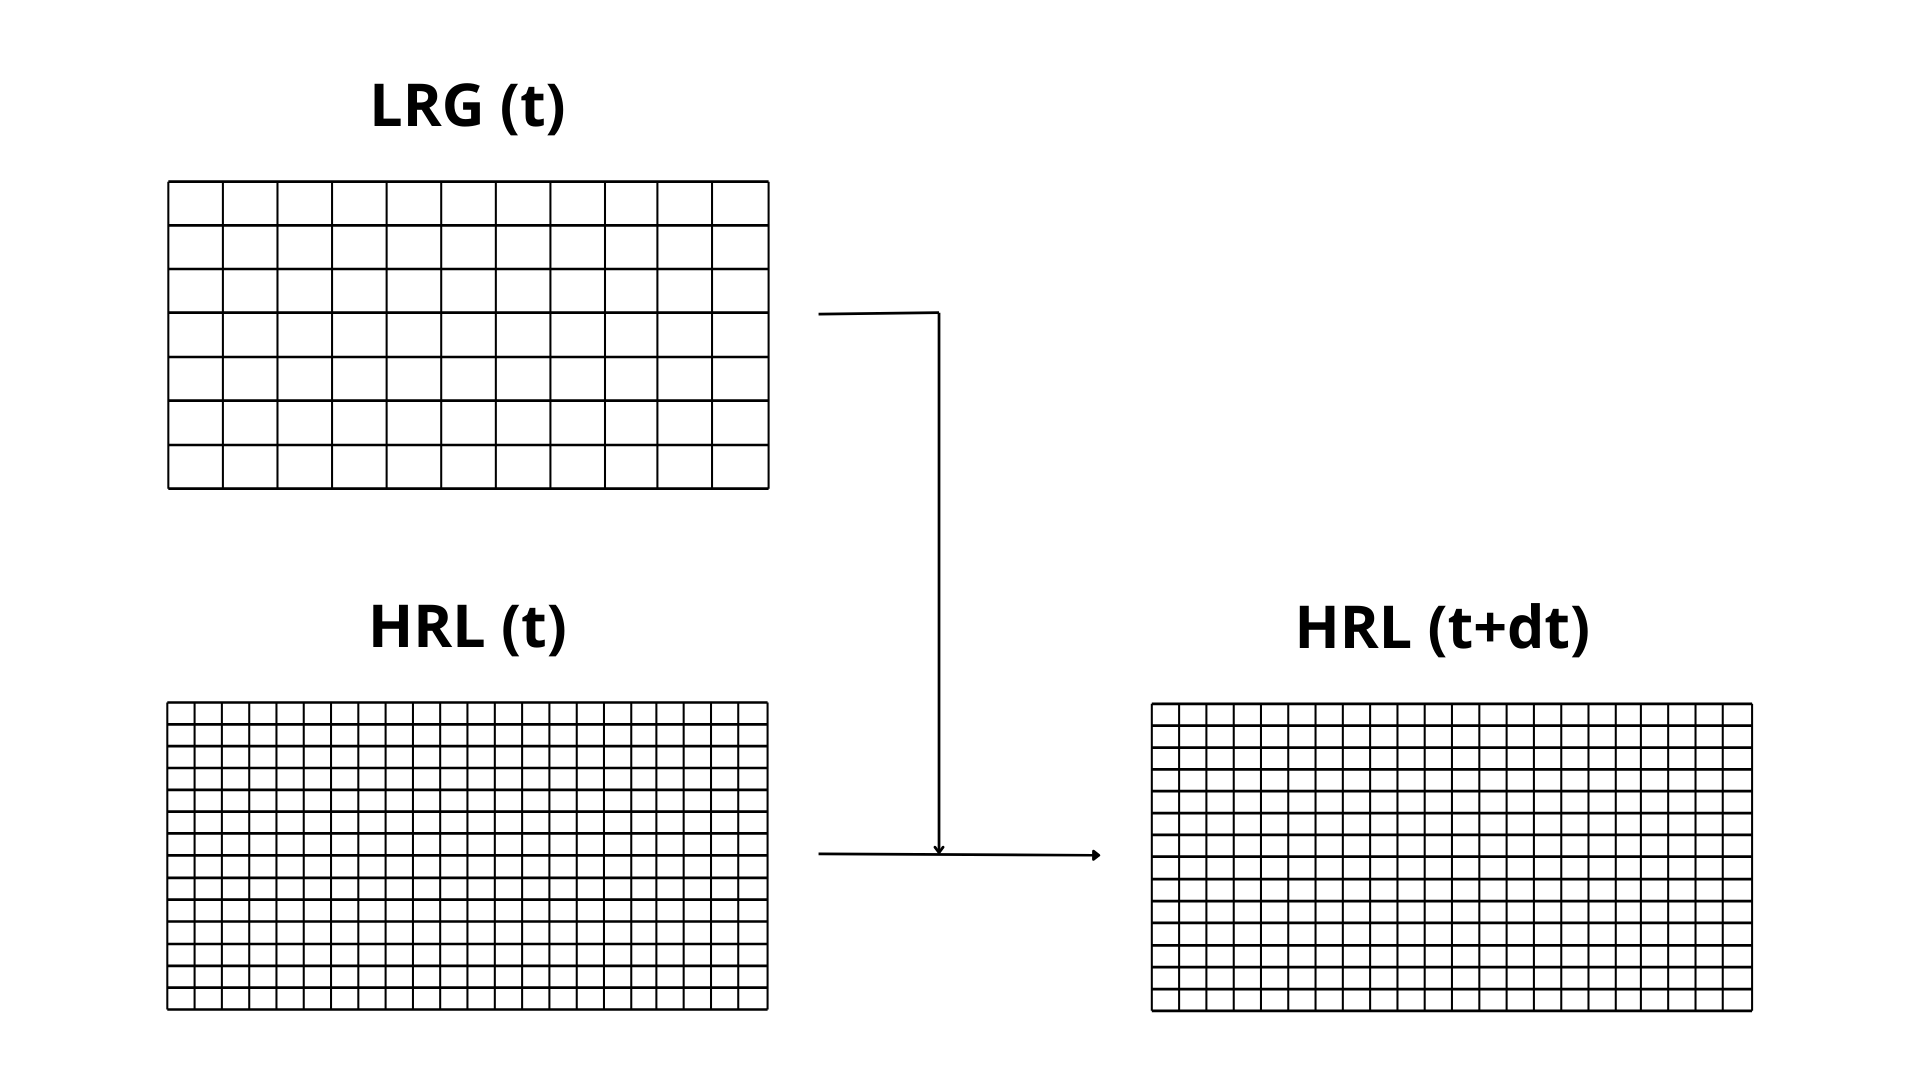
\includegraphics[width=0.9\textwidth]{media/model2.png}
\caption{Architecture of Model 2: Forecast with Degraded Boundary Conditions}
\label{fig}
\end{figure}

The objective of this model is to test whether having a broader system state at time t (boundary conditions) with lower resolution can yield better results for the local high-resolution domain at time t+dt.

\subsection{Model 3: Forecast and Downscaling}

\begin{figure}[ht]
\centering
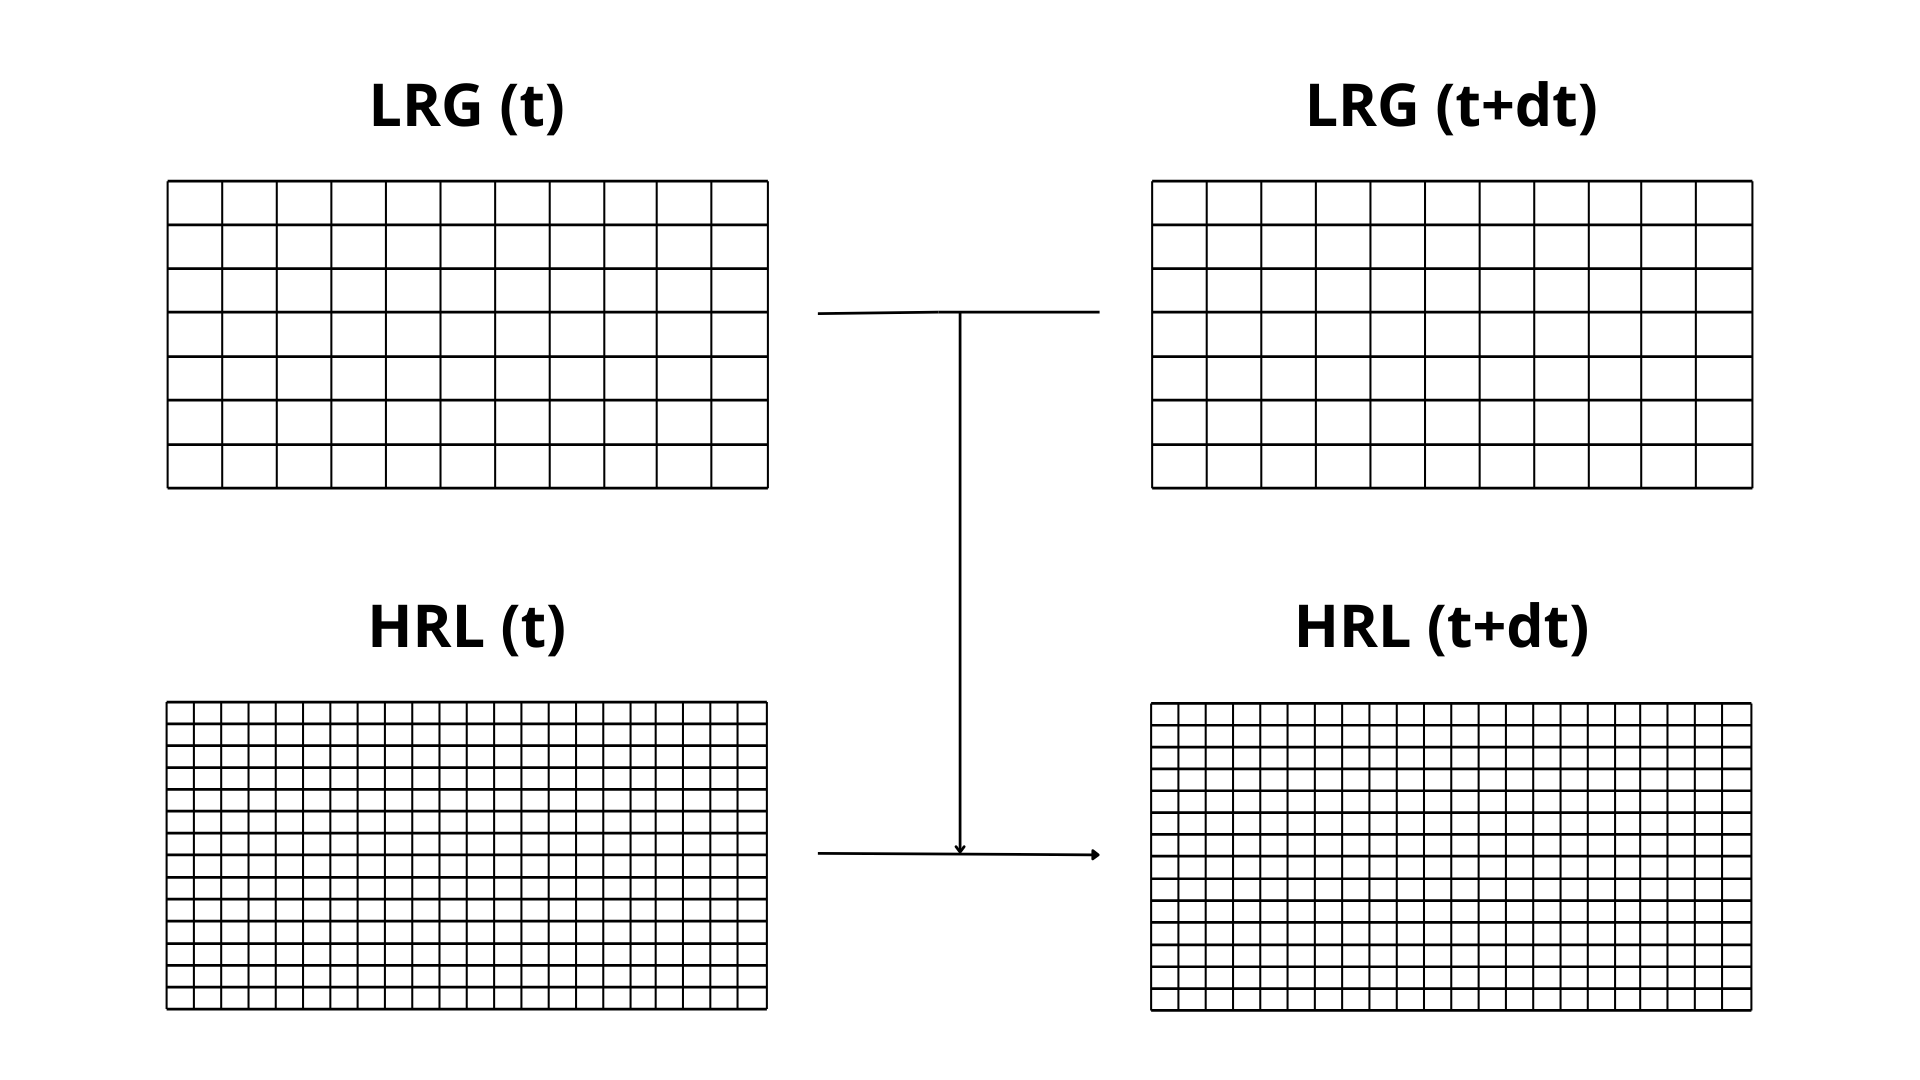
\includegraphics[width=0.8\textwidth]{media/model3.png}
\caption{Architecture of Model 3: Forecast and Downscaling}
\label{fig}
\end{figure}

The objective of this model is to test whether having a broader system state at both time t and time t+dt (the predicted time) with lower resolution can yield better results for the local high-resolution domain at time t+dt. This model involves both forecasting and downscaling steps.

\subsection{Model 4: Rollout or Autoregressive}

\begin{figure}[ht]
\centering
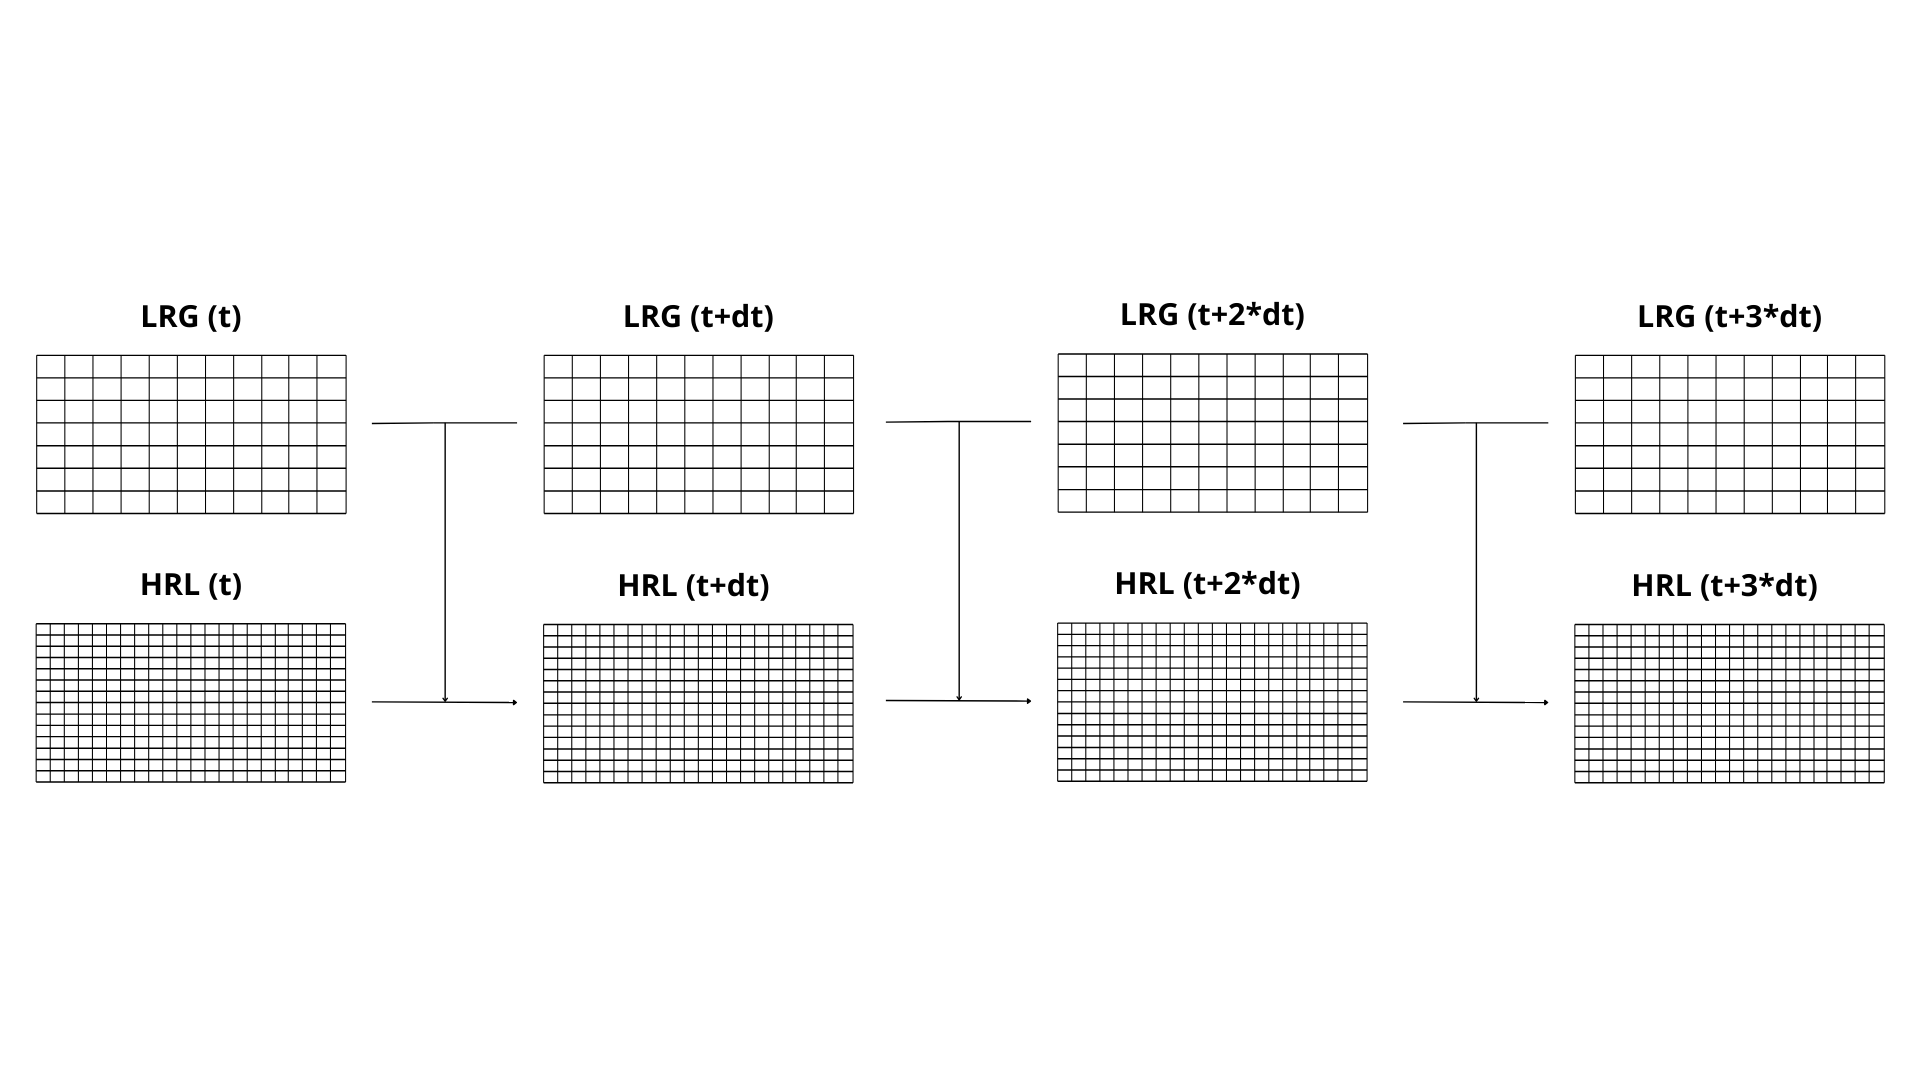
\includegraphics[width=0.9\textwidth]{media/model4.png}
\caption{Architecture of Model 4: Rollout}
\label{fig}
\end{figure}

The output from the previous iteration becomes the new input. The goal is to test the model's ability to predict an output at time n without significant error accumulation.
\newpage

\chapter{State of the art model}

\section{Spatial Resolution}

\begin{tabular}{>{\bfseries}l<{\hspace{1em}} >{\raggedleft\arraybackslash}p{5cm}}
\hline
\textbf{Model} & \textbf{Resolution} \\
\hline
Keisler \cite{keisler} & 1° * 1°\\
Pangu Weather \cite{panguweather} & 0.25° * 0.25° \\
Pangu Weather lite \cite{panguweather} & 0.25° * 0.25° \\
GraphCast \cite{graphcast} & 0.25° * 0.25° \\
GraphCast Small \cite{graphcast} & 1° * 1° \\
FuXi \cite{fuxi} & 0.25° * 0.25° \\
KARINA \cite{Karina} & 2.5° * 2.5° \\
\end{tabular}

\vspace{2em}
An interesting aspect of Keisler's approach is that he initially trained his neural network on input data with a resolution of 2 degrees for 3.5 days using a learning rate (lr) of 3e-4. Subsequently, the network was trained on data with a resolution of 1 degree for 1 day with lr=3e-5, followed by another day of training with lr=3e-6.

\section{Time Resolution}

\begin{tabular}{>{\bfseries}l<{\hspace{1em}} >{\raggedleft\arraybackslash}p{5cm}}
\hline
\textbf{Model} & \textbf{Time step (in hour)} \\
\hline
Keisler & 6 \\
Pangu Weather &  1,3,6,24 \\
Pangu Weather lite &  24 \\
GraphCast & 6 \\
GraphCast small & 6 \\
FuXi & 6 \\
KARINA & 24 \\
\end{tabular}

\vspace{2em}
Interestingly, FuXi's study builds on a comment made in the Pangu Weather paper, which notes that for a 7-day weather forecast, it is more accurate to run a 24-hour model seven times than to run a 1-hour model 168 times. This significantly reduces error accumulation. However, training a model for more than 24 hours is challenging. FuXi has developed both deterministic and ensemble versions of their model to address this challenge.

\section{Code availablity}

\begin{tabular}{>{\bfseries}l<{\hspace{1em}} >{\centering\arraybackslash}p{6cm} >{\raggedleft\arraybackslash}p{5cm}}
\hline
\textbf{Model} & \textbf{Code} & \textbf{Pre-trained}\\
\hline
Keisler & Yes \cite{keiser-github} & No \\
Pangu Weather &  Yes \cite{pangu-weather-Github} & Yes \\
Pangu Lite &  Yes \cite{pangu-weather-Github} & Yes \\
GraphCast & Yes \cite{graphcast-github} & Yes \\
GraphCast small & Yes \cite{graphcast-github} & Yes \\
FuXi & \textcolor{red}{No} \cite{fuxi-repo} & Yes \\
KARINA & \textcolor{green}{Yes} \cite{karina-code} & \textcolor{green}{Yes} \\
LAM & \textcolor{green}{Yes} \cite{neural-lam} & \textcolor{green}{Yes}
\end{tabular}

\vspace{2em}
GraphCast small has a resolution of 1°, 13 pressure levels, and trained on ERA5 data from 1979 to 2015 instead of 0.25 degree resolution, 37 pressure levels), trained on ERA5 data from 1979 to 2017.\\
Pangu Lite has only been trained and tested in 00UTC data and on 11 years instead of 39 years.

\section{Training Time with Different Models}

\begin{tabular}{>{\bfseries}l<{\hspace{1em}} >{\centering\arraybackslash}p{6cm} >{\raggedleft\arraybackslash}p{5cm}}
\hline
\textbf{Model} & \textbf{Number of GPUs} & \textbf{Training Time}\\
\hline
Keisler & 1 Nvidia A100 GPU & 5.5 days \\
Pangu Weather &  192 Nvidia Tesla-V100 GPUs & 4 * 16 days \\
GraphCast & 32 Google Cloud TPU v4 devices & 4 weeks \\
FuXi & 8 Nvidia A100 GPUs & 30 hours \\
KARINA & 4 Nvidia A100 GPUs & 12 hours \\
\end{tabular}

\newpage
\section{Keisler with Graph Neural Networks}

\subsection{Machine Learning Architecture}

\begin{figure}[ht]
\centering
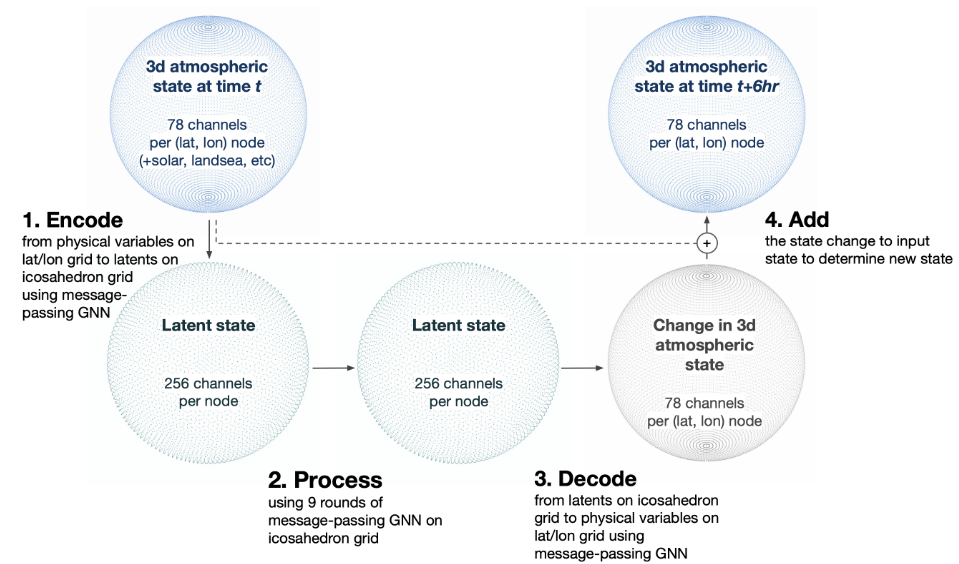
\includegraphics[width=0.9\textwidth]{media/Keisler_archi.png}
\caption{Keisler Model Learning Architecture}
\label{fig}
\end{figure}

The model employs Graph Neural Networks (GNNs) and is inspired by the approach of Pfaff et al. \cite{pfaff}. The GNN parameters are learned using historical training data (ERA5), leveraging the JAX library and two JAX-based packages: Jraph for constructing the GNN structures and Haiku for managing the neural networks themselves.

The model architecture is presented as follows: three main components - an encoder, a processor, and a decoder. The encoder maps the data from the native space (physical data on a latitude/longitude grid) to an intermediate space (abstract feature data on an icosahedral grid), while the processor handles this data in the intermediate space and the decoder maps the results back to the native space.

The use of an icosahedral grid for the intermediate representation is motivated by the fact that it provides a more uniformly distributed and efficient processing grid than the original latitude/longitude grid. The H3 package is used to define an icosahedral grid of level 2, which consists of 5,882 nodes (compared to 65,160 in the original lat/lon grid) with an angular separation of 3 degrees (approximately 330 km) between the nodes.

Each of the three components of the model is implemented as a message-passing GNN, using 2-layer MLPs with ReLU activation, LayerNorm, and 256 output channels for the neural networks.

\subsection{Data Availability}

All codes are available on this \href{https://github.com/openclimatefix/graph_weather/tree/main}{GitHub repository}.

\newpage
\section{Lam with GraphCast}

\subsection{Machine Learning Architecture}

The GraphCast system is a machine learning architecture that takes as input the two most recent states of the Earth's weather (the current time and six hours prior) and predicts the next state of the weather six hours in advance. A single weather state is represented by a latitude/longitude grid of 0.25° (721 x 1440), which corresponds to a resolution of approximately 28 x 28 kilometers at the equator, where each grid point represents a set of surface and atmospheric variables. GraphCast is autoregressive, meaning it can be "unrolled" by feeding its own predictions back into the input to generate an arbitrarily long trajectory of weather states.\\

GraphCast is implemented as a neural network architecture based on GNNs in an "encode-process-decode" configuration, with a total of 36.7 million parameters. The encoder uses a single GNN layer to map variables (normalized to zero mean and unit variance) represented as node attributes on the input grid to learned node attributes on an internal "multi-mesh" representation. The multi-mesh is a spatially homogeneous graph with high spatial resolution on the globe, defined by iteratively refining a regular icosahedron (12 nodes, 20 faces, 30 edges) six times, where each refinement divides each triangle into four smaller ones and reprojects the nodes onto the sphere.\\

The processor uses 16 unshared GNN layers to perform efficient local and long-range information propagation with few message passing steps on the multi-mesh. The decoder maps the learned features from the last layer of the processor from the multi-mesh representation to the latitude-longitude grid and predicts the output as a residual update of the most recent input state (with output normalization to achieve unit variance on the residual target).\\

During model development, 39 years (1979-2017) of historical data from the ECMWF's ERA5 reanalysis archive were used. GraphCast was trained to minimize the training objective using gradient descent and backpropagation. Training GraphCast took approximately four weeks on 32 Cloud TPU v4 devices using batch parallelism.\\

\subsection{Data Availability}

The code is available \href{https://github.com/google-deepmind/graphcast}{here}. The model is available pre-trained, as well as a smaller model with lower resolution.

\newpage
\section{Keifeng with Pangu-Weather}

\subsection{Machine Learning Architecture}

The methodology involves training deep learning networks to take reanalysis weather data as input at a given point in time and produce reanalysis weather data at a future point in time as output. The team utilized a single point in time for both input and output. The temporal resolution of the ERA5 data is 1 hour, with up to 341,880 time points in the training subset (1979-2017), constituting the amount of training data in one epoch. To mitigate the risk of overfitting, the team randomly shuffled the order of samples from the training data at the beginning of each epoch.\\

The team trained four models with lead times (the difference in time between input and output) of 1 hour, 3 hours, 6 hours, and 24 hours, respectively. Each of the four models was trained for 100 epochs, with each taking approximately 16 days on a cluster of 192 NVIDIA Tesla-V100 GPUs.\\

The architecture is known as the 3D Earth-specific transformer (3DEST). The team incorporated all the weather variables included, such as 13 layers of upper-air variables and surface variables, into a single deep network. They then performed patch embedding to reduce the spatial resolution and combined the downsampled data into a 3D cube. The 3D data is propagated through an encoder-decoder architecture derived from the Swin transformer, a vision transformer variant, which has 16 blocks. The output is divided into upper-air variables and surface variables and is resampled with patch recovery to restore the original resolution. To inject Earth-specific priorities into the deep network, the team designed a position bias (a mechanism for encoding the position of each unit) to replace the original relative position bias of Swin. This modification increases the number of bias parameters by a factor of 527, with each deep 3D network containing approximately 64 million parameters.\\

The lead time of a medium-range weather forecast is 7 days or more. This prompted the team to call the base models (with lead times of 1 hour, 3 hours, 6 hours, or 24 hours) iteratively, using each predicted result as input for the next step. To reduce cumulative forecast errors, they introduced a hierarchical temporal aggregation, a 'greedy' algorithm that always calls the model with the largest possible lead time. Mathematically, this significantly reduces the number of iterations. For example, if the lead time were 56 hours, the team would run the 24-hour forecast model 2 times, the 6-hour forecast model 1 time, and the 1-hour forecast model 2 times (Figure 1b). Compared to FourCastNet, which uses a fixed 6-hour forecast model, the team's method is faster and more accurate.\\

\subsection{Data Availability}

The code is available but currently under review. The pre-trained model is also available, along with a lite version that has a 24-hour step and has been tested only on 00 UTC.\\

\newpage
\section{Chen with FuXi}

The aim of this paper is to mitigate the error in forecasts due to the low-step model used for long-range predictions (10 days).

\subsection{Machine Learning Architecture}

\begin{figure}[ht]
\centering
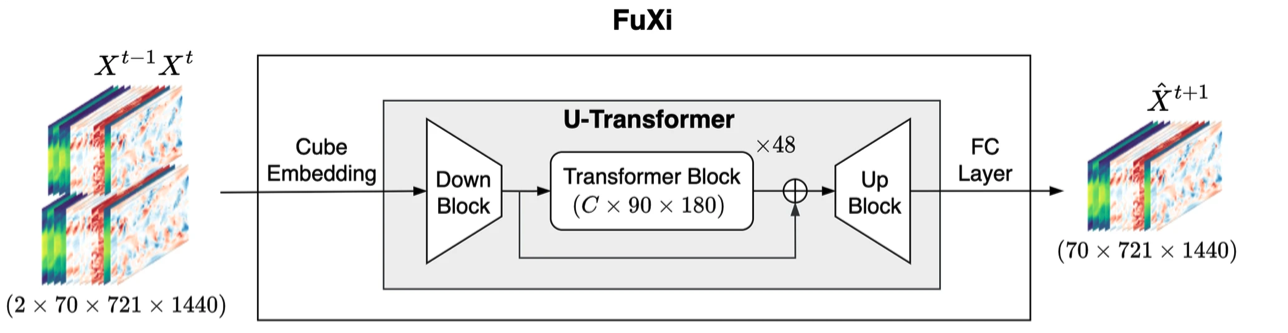
\includegraphics[width=0.9\textwidth]{media/FuXi_archi.png}
\caption{FuXi model learning architecture.}
\label{fig}
\end{figure}


\subsection{Data Availability}

The code for the model is available, albeit unreviewed. The pre-trained model is also available.

\newpage
\section{Cheon with KARINA}

KARINA is a machine learning model for global weather prediction that aims to be computationally efficient, particularly during training. It required 4 NVIDIA A100 GPUs for less than 12 hours of training. However, the model has a low resolution of 2.5 degrees. It utilizes 66 parameters, including 6 surface parameters and 5 atmospheric parameters, across 12 vertical isobaric layers from the surface to the lower stratosphere. The tensor has a dimension of 7214466. The low resolution is considered by the authors to be an effective means of extracting global patterns while smoothing noise.\\

\subsection{ML Architecture}

The model employs a ConvNext architecture with two innovations: SENet for dynamic parameter recalibration and the introduction of geocyclic padding to preserve continuity at 0° and 360°.\\

Squeeze-and-Excitation Networks (SENet) enable the model to focus on the most relevant features and meteorological variables through channel-wise recalibration.\\

Geocyclic Padding: Geocyclic padding handles the spherical topology by performing circular padding of the longitudinal edges and reorganizing the polar regions. This maintains geographic continuity.\\

\subsection{Data Availability}

The paper has been available for one month and has not yet been published in an official journal. The code has just been made available \href{https://github.com/jmj2316/KARINA/}{on this GitHub repository}.\\

\subsubsection{\href{https://github.com/jmj2316/KARINA/blob/main/networks/karina.py}{KARINA.py}}

Let's analyze the code named KARINA.py in detail:
This code is the body of the implementation of their CNN presented in the paper.\\

We can start with the functions:\\

\begin{itemize}
\item \textbf{SELayer(nn.Module)}: This class defines the Squeeze-and-Excitation Layer, which is the channel attention layer. An attention layer allows a CNN to "improve the representation of features." This class defines two functions:
\begin{enumerate}
\item \textbf{Init}: The class constructor takes two arguments: channel (the number of channels) and reduction, which I believe reduces the dimensionality of the data by a factor of 16. In this constructor, we find: mean pooling on the input data, a fully connected layer (all nodes in the layer connect to all nodes in the next layer) with ReLu and Sigmoid activation functions.
\item \textbf{Forward}: Applies mean pooling and then the fully connected layer to y, then multiplies the input tensor x by y, which is resized to match the size of x.
\end{enumerate}
\item \textbf{GeoCyclicPadding}: This class allows the innovation presented in the paper, i.e., to create a tensor that represents the constraint of a spherical domain. (I won't go into detail for now)
\item \textbf{Block}
\begin{enumerate}
\item \textbf{Init}: The class constructor with three arguments: dim, the input dimension, droppath, the dropout rate set to zero, and therefore this function is never used (i.e., the input tensor is transmitted without modification). It can prevent overfitting in some cases, but it does not seem to be used here. Otherwise, the rest of the function is intended to apply \textit{SELayer and GeoCyclic Padding}
\item \textbf{Forward}: The way x is propagated through a network.
\end{enumerate}
\item \textbf{ConvNext}:
\begin{enumerate}
\item \textbf{Init}: The class constructor with four arguments: the number of input channels (in chans), the number of output classes (num classes), the depths of the different blocks (depths), and the dimensions of the different blocks (dims). It initializes the downsampling layers (downsample layers) and the stages of the network using the Block defined above.
\item \textbf{init weights}: As the name suggests, it initializes the weights.
\item \textbf{forward features and forward}: The way x is propagated through the network.
\end{enumerate}
\item \textbf{Layer Norm}: As the name suggests, this class is used to normalize the network, layer by layer. It uses the layer norm function of PyTorch.
\item \textbf{KARINA}:
\begin{enumerate}
\item  \textbf{init} 5 arguments : the size of the image (img size), the number of input channels (in chans), the number of output channels (out chans), the depths of the different blocks (depths) and the dimensions of the different blocks (dims)
\item \textbf{forward} it propagates the network in convnext.
\end{enumerate}
\item \textbf{Main}: Defines the input and passes it through the model.
\end{itemize}

\subsubsection{\href{https://github.com/jmj2316/KARINA/blob/main/train_KARINA.py}{train-KARINA.py}}

Let's analyze in detail how the model is trained. \textbf{TO BE DONE LATER}\\

\begin{itemize}
\item \textbf{Set seed(seed)}: This function aims to define a SINGLE random number generator and thus to have reproducibility of results (by performing the same operation, we will get the same result). In this function, we define the "seed" for PyTorch CPU and GPU, for numpy random and classic random, for object hashing (not well understood here the interest). We define cuDNN as deterministic: convolution operations are therefore deterministic and reproducible. And we disable the \textbf{benchmark} option, which seems to automatically select convolution algorithms, and therefore, once again, in the interest of result reproducibility, we disable this option.
\end{itemize}

\newpage
\section{Limited Area Modelling}

This section follows up on a discussion initiated by Prof. Myoshi in Vienna \cite{Raynaud2024}. Upon conducting research, I came across a publication by Joel Oskarsson et al. \cite{LAM}. To deepen my understanding of this domain, I should read this \href{https://www.researchgate.net/publication/349484799}{chapter}.\\

The title of the article is "Graph-based Neural Weather Prediction for Limited Area Modeling." In this article, the authors present an implementation of a neural weather prediction system based on graph theory. The article describes three models: GC-LAM, 1L-LAM, and HI-LAM.\\

The first two models, GC-LAM and 1L-LAM, are direct implementations of the GraphCast model. In GraphCast, the boundaries of each node's domain have different resolutions, enabling the propagation of long-range physical phenomena while maintaining precision for local phenomena.\\

HI-LAM introduces an innovation by proposing different node architectures adapted to various resolutions. This approach addresses the problem of nodes having less information than others. In HI-LAM, all nodes receive the same information, eliminating certain artifacts along the edges of the nodes.\\

\begin{figure}[ht]
\centering
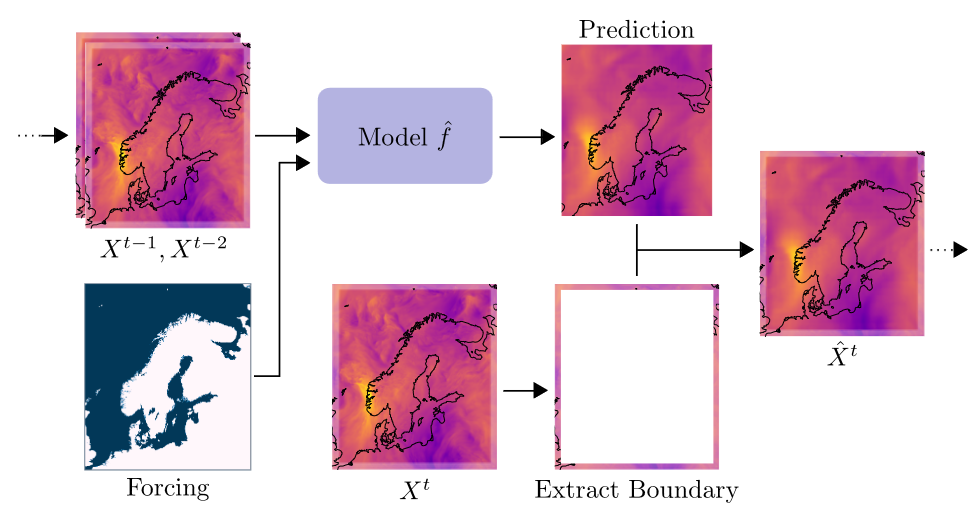
\includegraphics[width=0.9\textwidth]{media/LAM_Boundary-Forcing.png}
\caption{Boundary forcing in the case of a LAM}
\label{fig}
\end{figure}

A specific consideration is how the boundary conditions are obtained. To address this issue, before each iteration, an expanded domain is given to the algorithm to define the forcing (see figure \ref{fig}). One question that arises is whether this expanded domain is sufficient, or if a global model should be provided to the system for more relevant predictions. Furthermore, in an operational context, we would be required to use a global model to extract this information at each time step. Therefore, a low-resolution global model coupled with a high-resolution local model would be advantageous.



\chapter{Architecture}

\section{ConvNeXt}
ConvNeXt is a Fully Convolutional Neural Network (FCNN) presented in the paper "A ConvNet for the 2020s" \cite{liu2022convnet}. This network is utilized in the KARINA model and, according to its author, outperforms transformers on primary Vision testing metrics. The author details the roadmap used to modernize the architecture and surpass the current best transformer, SwinT, presented in \cite{liu2021swin}.

We will follow the author's roadmap to explain the modernization process and gain a better understanding of ConvNeXt's functionality.

\subsection*{Training Techniques}
The initial hypothesis is that the training procedure is one of the critical aspects to improve for achieving higher accuracy. The author suggests that transformer training procedures have been refined more and thus, applies a similar training procedure for ConvNeXt. Some of the changes include: increasing the number of epochs, using the AdamW optimizer, data augmentation techniques such as Mixup, Cutmix, RandAugment, Random Erasing, and regularization techniques including Stochastic Depth and Label Smoothing.

The author concludes that "a significant portion of the performance difference between traditional ConvNets and vision Transformers may be due to the training techniques."

A summary of the (pre-)training configuration can be found in Table \ref{tab:train_detail},and a summary of the fine-tuning configuration can be found in Table \ref{tab:ft_detail}.\\


\begin{table}[ht]
\tiny
\begin{minipage}{.55\linewidth}
\centering
\begin{tabular}{@{\hskip -0.05ex}l|c@{\hskip 1ex}c}
& ConvNeXt-T/S/B/L & ConvNeXt-T/S/B/L/XL \\
\multirow{2}{*}{(pre-)training config} & ImageNet-1K & ImageNet-22K \\
& 224$^2$ & 224$^2$ \\
\hline
weight init & trunc. normal (0.2) & trunc. normal (0.2) \\
optimizer & AdamW & AdamW\\
base learning rate & 4e-3 & 4e-3 \\
weight decay & 0.05 & 0.05 \\
optimizer momentum & $\beta_1, \beta_2{=}0.9, 0.999$ & $\beta_1, \beta_2{=}0.9, 0.999$ \\
batch size & 4096 & 4096 \\
training epochs & 300 & 90 \\
learning rate schedule & cosine decay & cosine decay \\
warmup epochs & 20 & 5 \\
warmup schedule & linear & linear \\
layer-wise lr decay  & None & None \\
randaugment  & (9, 0.5) & (9, 0.5) \\
mixup  & 0.8 & 0.8 \\
cutmix  & 1.0 & 1.0 \\
random erasing  & 0.25 & 0.25 \\
label smoothing  & 0.1 & 0.1 \\
stochastic depth & 0.1/0.4/0.5/0.5 & 0.0/0.0/0.1/0.1/0.2 \\
layer scale & 1e-6 & 1e-6 \\
head init scale  & None & None \\
gradient clip & None & None \\
exp. mov. avg. (EMA) & 0.9999 & None\\
\end{tabular}
\caption{\textbf{ImageNet-1K/22K (pre-)training settings}. Multiple stochastic depth rates (e.g., 0.1/0.4/0.5/0.5) are for each model (e.g., ConvNeXt-T/S/B/L) respectively.}
\label{tab:train_detail}
\end{minipage}%
\begin{minipage}{.4\linewidth}
\centering
\begin{tabular}{@{\hskip -0.05ex}l@{\hskip 2.6ex}|cc}
\multirow{2}{*}{fine-tuning config} & ImageNet-1K   & ImageNet-1K  \\
 & 384$^2$ & 224$^2$ and 384$^2$ \\
\hline
optimizer & AdamW & AdamW\\
base learning rate & 5e-5 & 5e-5 \\
weight decay & 1e-8 & 1e-8 \\
optimizer momentum & $\beta_1, \beta_2{=}0.9, 0.999$ & $\beta_1, \beta_2{=}0.9, 0.999$ \\
batch size & 512 & 512 \\
training epochs & 30 & 30 \\
learning rate schedule & cosine decay & cosine decay \\
layer-wise lr decay & 0.7 & 0.8  \\
warmup epochs & None & None \\
warmup schedule & N/A & N/A \\
randaugment & (9, 0.5) & (9, 0.5) \\
mixup & None & None \\
cutmix  & None & None \\
random erasing & 0.25 & 0.25 \\
label smoothing  & 0.1 & 0.1 \\
stochastic depth  & 0.8/0.95 & 0.0/0.1/0.2/0.3/0.4 \\
layer scale & pre-trained & pre-trained \\
head init scale & 0.001 & 0.001 \\
gradient clip & None & None \\
exp. mov. avg. (EMA) & None & None(T-L)/0.9999(XL) \\
\end{tabular}
\caption{\textbf{ImageNet-1K fine-tuning settings}. Multiple values (e.g., 0.8/0.95) are for each model (e.g., ConvNeXt-B/L) respectively. }
\label{tab:ft_detail}
\end{minipage}
\end{table}



\newpage
\subsection*{Macro design}

The autors made two main changes to the design wich are \textbf{Changing stage} compute ratio and \textbf{Changing stem to “Patchify”}. We will go trough them.\\

The stages of the computation are a macro design choice. The stage are blocks of operation done in order they often reflect the end goal of the Neural Network. \textit{Changing stage} here means changing the number of time one block is computed at each stage. For reference the old ResNet had a compute factor of [3,4,6,3] after the stem layer and SwinT has a ratio of [1,1,3,1] and for larger transformer [1,1,9,1]. Following this architecture the author proposed a new one following the first ratio [3,3,9,3]. It has improved the accuracy of the model but the author points out that a better design is likely to exist.\\

The stem layer is design to adapt the image for the processing in the network in computer vision there are a lot of redundancy is the image and that is why the stem layer has the role of downsampling the input image. One main difference with transformer is the rate of the downsampling, for convNet the rate is 4 time and SwinT has a rate of 14. The convolution layer of the standard resNet is 7*7 when SwinT has a 4*4. The stem layer of the new convNet is now 4*4 with a stride of 4 (previously the stride was 2) to augment the downsampling. The authors use what the call the “patchify stem” (4×4 non-overlapping convolution) in the network.\\

\subsection*{Grouped convolution}

The idea here was to implement what had been done in other convolutionnal network to have a better trade-off Flops/accuracy. The guiding principle is to “use more groups, expand width”. The idea here is to use depth-wise convolution, a grouped convolution where the number of groups equals the number of channels. The combination of depth-wise conv and 1 × 1 convs leads to a separation of spatial and channel mixing, a property shared by vision Transformers, where each operation either mixes information across spatial or channel dimension, but not both. By doing so the Flops are reduced and they increased the network width to the same number of channels as Swin-T’s (from 64 to 96)
to return to the same amount of Flops.

\subsection*{Inverted Bottleneck}

One major difference between classical ConvNet and Transformer is the use of inverted bottleneck for the latter. Inverted bottleneck is a technique where the "hidden" dimension of the MLP is wider than the input and output. This opperation improved the performance and decrease the Flops which is quite a fun result.

\subsection*{Large Kernel Sizes}

One of the most distinguishing aspects of vision Transformers is their non-local self-attention, which enables each layer to have a global receptive field. For SwinT the self attention layer is has a window size of 7*7 contrary to 3*3 for classical resNet. To explore large kernels, one prerequisite is to move up the position of the depthwise conv layer. In transformers the Multi-Head Self Attention (MSA) Layer is placed ahead of the MLP. They tested multiple size of window and found that the best one was 7×7 depthwise conv in each block.

\subsection*{Micro Design}

The first micro design change that they made was to substituted ReLU activation function with GELU. The second change they made was to have the same number of activation function as the transformer wich is one per MLP. So they have only kept the on GELU function between the two one by  one layer. Again the removed normalisation layer that are less present in transformers. They only kept one BatchNorm (BN) before the one by one conv layer. They now have less normalisation function than the transformers because they empirically found that it works best. They then changed BN for Layer Normalisation (LN) wich is mostly used in transformers and found a slight increase in performance. They used 2*2 conv layer with stride 2 for downsampling between each stage and added LN for stabilising the result (one before each downsampling layer, one after the stem, and one after the final global average pooling).
\newpage

\section{Graph Neural Networks}

Graph Neural Networks (GNNs) are a class of neural networks that operate directly on graph data structures. They have emerged as a powerful tool for machine learning based Weather Prediction. One of the first MLWP was made using this type of architecture \cite{keisler} and after that GraphCast also used this architecture. 

\subsection{Overview of GNNs}

GNNs extend the neural network concepts to graph data by learning to capture the dependencies between connected nodes. They do so by passing messages or information along the edges of the graph, updating the representation of each node based on the representations of its neighbors. This process is often referred to as message passing or neighborhood aggregation.

\subsection{Message Passing in GNNs}

In a typical GNN, each node is initialized with a feature vector, and the goal is to learn a new representation for each node that captures both its own features and the features of its neighbors. This is achieved through a series of message passing steps, where each node aggregates the feature vectors of its neighbors and updates its own feature vector based on the aggregated result.\\

Formally, the update rule for a node $v$ at the $k$-th iteration can be written as:\\

$$h_v^{(k)} = \text{UPDATE}\left(h_v^{(k-1)}, \text{AGGREGATE}\left(\left\{h_u^{(k-1)}: u \in \mathcal{N}(v)\right\}\right)\right)$$

where $h_v^{(k)}$ is the feature vector of node $v$ at iteration $k$, $\mathcal{N}(v)$ is the set of neighbors of node $v$, and UPDATE and AGGREGATE are differentiable functions that can be learned during training.

\subsection{Learning More About GNNs}

For a more in-depth introduction to GNNs, go through this paper : \href{https://distill.pub/2021/gnn-intro/}{Graph Neural Networks: An Intuitive Introduction}.

\newpage

\section{Transformers}

It is impossible to discuss Transformers without referring to the seminal work "Attention is All You Need" \cite{vaswani2023attention}.\\

The Transformer architecture, proposed by Vaswani et al., revolutionized the field of natural language processing by introducing a model that relies entirely on attention mechanisms, dispensing with recurrence and convolutions. This shift allowed for more parallelization and significant improvements in computational efficiency.\\

The Transformer model is composed of an encoder and a decoder, each of which is a stack of identical layers. The primary innovation is the self-attention mechanism, which allows the model to weigh the importance of different vectors in the input sequence when producing an output. \\

The self-attention mechanism is complemented by positional encoding, which injects information about the relative or absolute position of the tokens in the sequence. This is crucial because, unlike recurrent neural networks, Transformers do not inherently capture the order of the input sequence.\\

In addition to self-attention, each layer in the Transformer includes a feed-forward neural network and normalization steps. Residual connections are employed around each sub-layer, followed by layer normalization, which helps to stabilize the learning process.\\

Let us look at this figure which was found in the paper by Vaswani et al.:\\

\begin{figure}[ht]
    \centering
    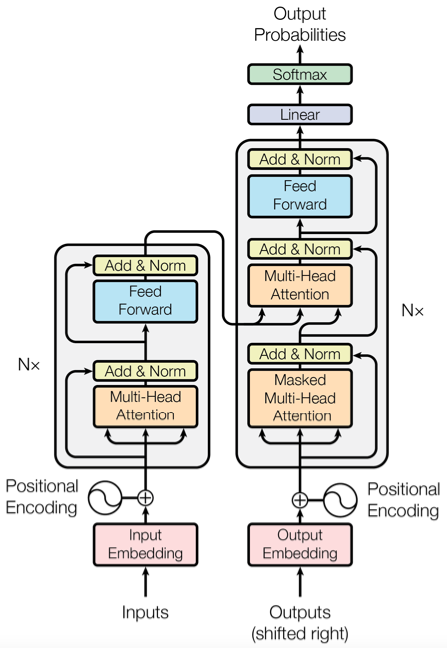
\includegraphics[width=0.4\textwidth]{media/Architecture_transfo.png}
    \caption{architecture of a transformer}
    \label{fig:transfo}
\end{figure}

\subsection{ViT}

ViT, or Vision Transformer, is a type of Transformer model that has been adapted for computer vision tasks \cite{dosovitskiy2021image}. \\

In the ViT model, an image is split into fixed-size patches, which are then linearly embedded. The resulting vectors serve as the input to the Transformer, similar to how word embeddings are used in NLP tasks. The key insight is that the self-attention mechanism can be used to model relationships between these image patches, much like it models relationships between words in a sentence.\\

The ViT model also uses positional embeddings to retain spatial information about the patches, similar to how positional encoding is used in the original Transformer. The output of the Transformer is then passed through a linear layer to produce the final image classification.\\

The ViT model has been shown to perform competitively with state-of-the-art convolutional neural networks on various image classification benchmarks. This demonstrates the versatility of the Transformer architecture and suggests that it could be a promising direction for future research in computer vision.\\

\subsection{Swin Transformer}

The Swin Transformer, introduced by Liu et al. \cite{liu2021swin}, is a hierarchical Transformer whose representation is computed using shifted windows. This model aims to address the issue of quadratic complexity with respect to the image size in standard Transformers by limiting self-attention computation to non-overlapping local windows. The shifted window approach allows for cross-window connections, enabling the modeling of long-range dependencies while maintaining computational efficiency.\\

\subsection{U-Transformer}

The U-Transformer is a variation of the Swin Transformer and is constructed using 48 repeated Swin Transformer V2 blocks. This model leverages the strengths of the Swin Transformer, such as its ability to model long-range dependencies efficiently, and combines them with a U-Net like architecture to provide a powerful tool for tasks requiring detailed, high-resolution output, such as semantic segmentation.\\

\newpage

\section{Fourier Neural Operator}

Fourier Neural operator have been implemented in MLWP since the start with FourCastNet. There are two main paper that i used for this review
\newpage

\chapter{Model Implementation}

In this chapter, I will detail the various changes and adjustments made to the original architectures of KARINA and ConvNext to better suit a local model at a resolution of 0.25°. The aim is to develop a regional machine learning weather prediction model that leverages the strengths of both KARINA and FourCastNet.\\

The original KARINA architecture was designed for global weather prediction and thus, certain modifications are necessary to adapt it to a regional model. Similarly, while ConvNext is a state-of-the-art convolutional neural network, it "may" requires modifications to be applicable to our specific use case.\\

In the following sections, I will provide a detailed explanation of each modification made to the original architectures and the rationale behind them. By the end of this chapter, we will have a clear understanding of how the original architectures were adapted to create a regional machine learning weather prediction model.\\

As viewed in the introduction on the section "models", the first implementation is "simply" a local forecast with as input the regional state at time t and as output that same regional state at time t+dt (6h).\\

Model0 is the playground of that first model where i try to understand how and what are the possiblities to adapt KARINA's model to a local model.\\

\section{Model 0}

In this section, I present the first attempt at creating a regional machine learning weather prediction model. This approach is based on the work done by KARINA and FourCastNet, but we will modify their code to adapt it to our regional modeling needs.\\

\subsection*{Padding}

One of the key modifications we need to make is to change the padding used in the convolutional layers. In KARINA's code, they used a cyclic padding approach, which was a significant improvement for global representation. However, in our case, we are working with a local model, and the earth deformation can be neglected. Therefore, we will not use the cyclic padding approach.\\

The padding is defined in the function \textbf{GeoCyclicPadding}. To modify it, we will need to remove the cyclic padding and replace it with a different padding approach. One important consideration is that when a convolutional filter is applied to an image, it may lose information at the edges. To avoid this, we will create a new padding function that we will call \textbf{LinearPadding}.\\

There are several choices for padding, including:\\

\begin{itemize}
\item \textbf{Zero padding:} This is the most common padding approach, where zeros are added to the edges of the image. This ensures that the convolutional filter can be applied without losing any information. However, it may introduce some bias towards zero in the output. Seen here \cite{padding2002}.
\item \textbf{Constant padding:} This approach involves adding a constant value to the edges of the image. The value can be chosen based on the application. For example, in image segmentation, a constant value of -1 can be used to indicate the background.
\item \textbf{Reflection padding:} This approach involves reflecting the image at the edges. This can help to preserve the structure of the image at the edges, but may introduce some artificial symmetry.
\item \textbf{Replication padding:} This approach involves replicating the values at the edges of the image. This can help to preserve the structure of the image at the edges, but may introduce some artificial repetition.
\end{itemize}

In our case, we will use zero padding, as it is the most common approach and has been shown to work well in many applications.\\

The new padding function will be defined as follows:\\


\begin{lstlisting}[language=Python, frame=single, basicstyle=\ttfamily\small, backgroundcolor=\color{red!10}]
class GeoRectangularPadding(nn.Module):
    def __init__(self, pad_width):
        super(GeoRectangularPadding, self).__init__()
        self.pad_width = pad_width

    def forward(self, x):
        batch_size, channels, height, width = x.shape

        # Rectangular padding for left and right
        left_pad = torch.zeros(batch_size, channels, height,
        self.pad_width, device=x.device)
        right_pad = torch.zeros(batch_size, channels, height,
        self.pad_width, device=x.device)
        left_right_padded = torch.cat([left_pad, x, right_pad],
        dim=3)

        # Rectangular padding for top and bottom
        top_pad = torch.zeros(batch_size, channels,
        self.pad_width, left_right_padded.shape[3], 
        device=x.device)
        bottom_pad = torch.zeros(batch_size, channels,
        self.pad_width, left_right_padded.shape[3], 
        device=x.device)
        top_bottom_padded = torch.cat([top_pad, left_right_padded,
        bottom_pad], dim=2)

        return top_bottom_padded
\end{lstlisting}


In this code, we create a new class called \textbf{GeoRectangularPadding}, which takes a padding width as input. The forward function adds zero-padding to the left, right, top, and bottom of the input tensor. The resulting tensor has the same shape as the input tensor, but with additional zeros at the edges. This new padding function will be used in place of the \textbf{GeoCyclicPadding} function in KARINA's code.\\

By using this linear padding approach, we can ensure that the convolutional filter can be applied to the image without losing any information at the edges. This modification is an important step in adapting KARINA's code for our regional modeling needs.\\

\subsection*{Input Size}

The actual input size is \textbf{(72, 144, 67} and we want to change that to \textbf{80,120,67} representing \textbf{lon ,lat, variables}.
\newpage

\chapter{Limitations of Machine Learning approaches}

This chapter is mostly based on the report of the ECMWF \cite{riseofdatadriven} published in the Bulletin of the American Meteorological Society. This paper is an assessment of Pangu weather vs ECMWF IFS in an operational-like context. What has been shown in that paper is an overly smooth forecast and under-representation of extreme events  creating Increasing biais with rollout and a poor performance in predicting tropical cyclone. The main reason for these problems is that the loss is a Root Mean Square Error. In previous studies, there has been a concern that training towards RMSE results in overly smooth forecast fields (see for example the smooth forecasts shown in \cite{keisler}).\\

Indeed, the RMSE strongly penalizes large forecast departures from the observations (or analyses), thus discouraging bold forecasts. When comparing RMSE from different models, it is therefore important to check the level of activity of the different forecasts while interpreting the results. The activity of a forecast is here defined as standard deviation of the forecast anomaly.

\section{Loss function}

The loss function is a RMSE for every paper that has been reviewed 


\printbibliography

% Table des figures
\listoffigures
\newpage

\appendix
\begin{landscape}
\begin{table}[htbp]
\centering
\setlength{\tabcolsep}{15pt}
\renewcommand{\arraystretch}{1.5}
\begin{tabularx}{\textwidth}{>{\bfseries}l<{\hspace{1em}} >{\centering\arraybackslash}X >{\centering\arraybackslash}X>{\centering\arraybackslash}X >{\raggedleft\arraybackslash}X}
\toprule
\thead{Model} & \thead{Resolution} & \thead{Time step\\(in hour)} & \thead{Code} & \thead{Architecture} \\
\midrule
Keisler \cite{keisler} & 1° * 1° & & & \\
Pangu Weather \cite{panguweather} & 0.25° * 0.25° & & & \\
GraphCast \cite{graphcast} & 0.25° * 0.25° & & & \\
FuXi \cite{fuxi} & 0.25° * 0.25° &  & & \\
KARINA \cite{Karina} & 2.5° * 2.5° & & & \\
FourCastNet \cite{pathak2022fourcastnet} & 0.25*0.25 & & & \\
\bottomrule
\end{tabularx}
\end{table}
\end{landscape}
\end{document}
